\section{Introduction}
The \ac{TCA} implementation for the \ac{CMR} is one that heavily utilizes geometry and a rigid-body model assumption, while also placing an emphasis on relying on minimal assumptions/data about the environment and avoiding computationally complex calculations on input data from sensors, cameras, etc. There were various reasons as to why some of these assumptions/choices were made and why the agreed upon implementation was deemed the best choice for the given scenario. \cite{tractl} Figure~\ref{traction_control:algorithms:scarecrow} shows a testbed version of the \ac{CMR}.

\begin{figure}[htbp]
	\centering
	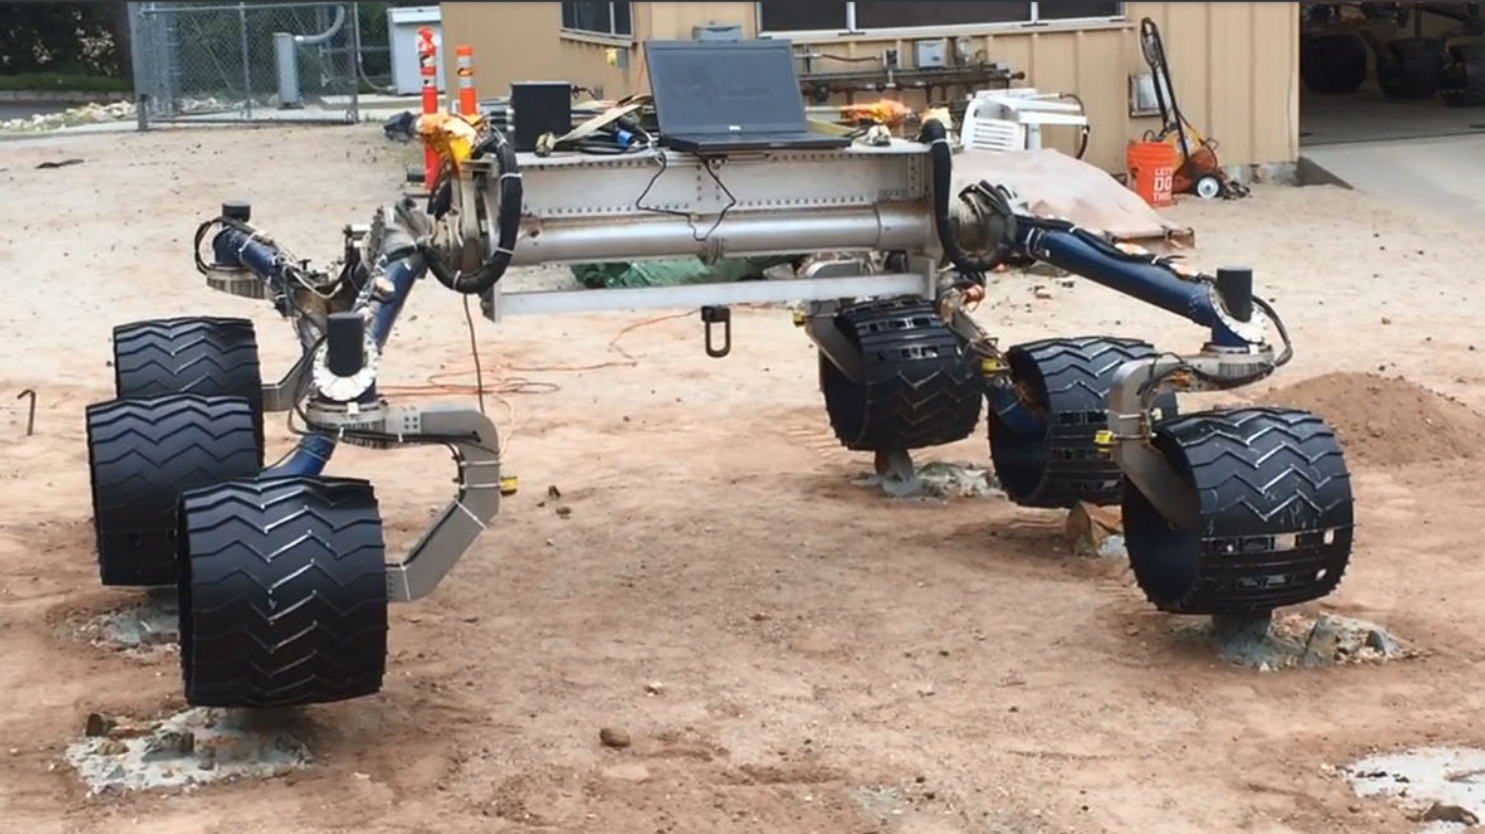
\includegraphics[width=.9\textwidth]{sections/algorithms/images/scarecrow_testbed.png}
	\caption{The Scarecrow Testbed Rover, a Rover Kinematically Similar to the \acl{CMR} \cite{tractl}}
	\label{traction_control:algorithms:scarecrow}
\end{figure}

\section{Design Limitations and Considerations}
It is important to note that the need for this \ac{TCA} was not discovered until after the flight system was actively engaging in its mission on the Martian surface, while ground control was observing telemetry of its use. Therefore, it was impossible to make any physical modifications to the \ac{CMR}, only software could be remotely flashed to it. \\

However, there are still ramifications to having this additional routine run on the \ac{CMR}. The limited computational resources available to do so must be considered carefully, so as to not interfere with existing processes being ran, and the implementation chosen has to have enough resources to perform the task it needs to as well. The team responsible for solving the problem at hand clarified some of these issues and how it restricted their choices for strategies to solve the problem. For example, the rover ``does not include force or torque sensors on the mobility subsystem, nor can it measure slip with high enough frequency to be able to react to it.'' \cite{tractl} \\

Some of the characteristics and assumptions of the \ac{CMR} and its \ac{TCA} implementation are discussed in the following sections.

\section{Ackermann Steering Model}
Modeling vehicles using the Ackermann steering model is a common practice, including for the \ac{CMR}. Even thought it adds slightly more complex geometric modeling, the mechanical steering system can be implemented relatively easily, and there are benefits to doing so. \\

Figure~\ref{traction_control:algorithms:ackermann-steering} illustrates a basic vehicle that is modeled using Ackermann steering, where the left image has the wheels positioned such that the vehicle will move straight, while the right image would cause the vehicle to turn counter-clockwise. Important to note is that when in a turning position, the front wheels are not turned to the same angle as one another, because of the nonzero distance between them. They are positioned such that the direction that both wheels are pointing are normal to a common center point called the \ac{ICC}, so that when the vehicle turns, the left and right wheels follow two different circular arcs, but both of their centers are at the \ac{ICC}.

\begin{figure}[H]
	\centering
	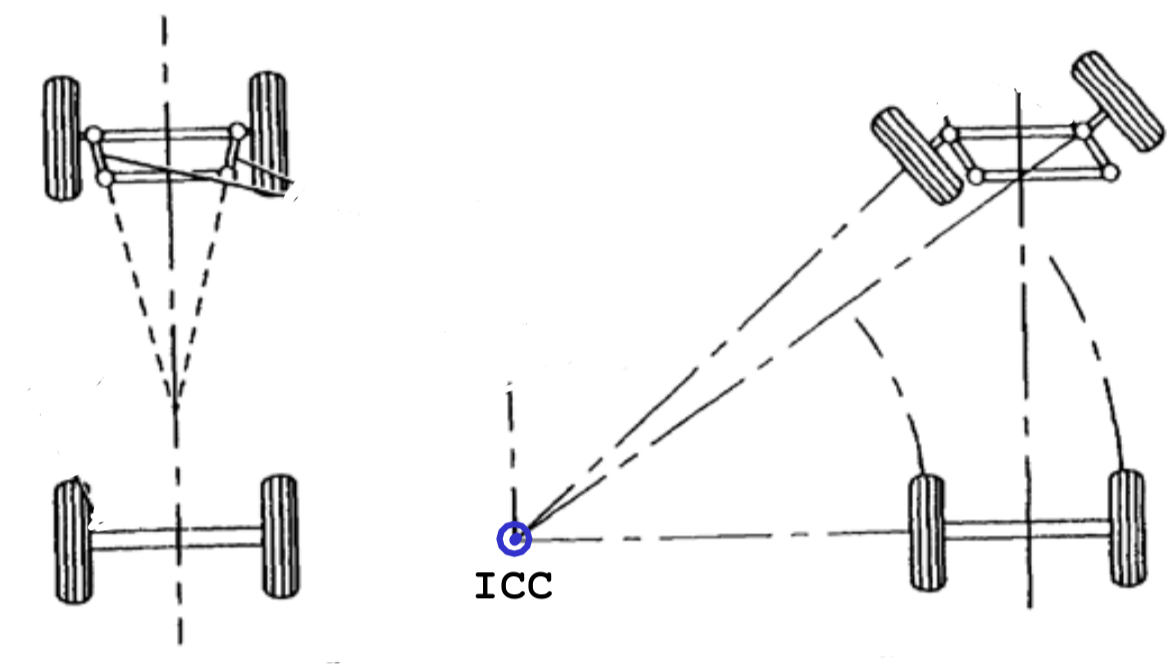
\includegraphics[width=.9\textwidth]{sections/algorithms/images/ackermann_steering.png}
	\caption{A Vehicle with Ackermann Steering Going Straight (Left) and in a Turning Position(Right)}
	\label{traction_control:algorithms:ackermann-steering}
\end{figure}

The benefit to this is that, assuming all the wheels' velocities are coordinated and in an ideal world, at no point while traveling in these flat, circular arcs will a wheel slip. Less slippage means less unpredictable behavior, such as a wheel slipping over a rough surface. However, the assumption that the \ac{CMR} would only be traversing terrain that could be modeled as flat is what led to the need for the \ac{TCA}, as excessive slippage occurred due to the reality that the terrain was non-negligible. As one wheel would traverse over a rock and then back down, it traveled a longer distance. \\

The Ackermann steering model by itself does not account for this extra distance and this caused the wheel slippage, which damaged them at an alarming rate. This is how the \ac{TCA} can be used to improve the model, so that when rough terrain is being traversed, the wheel(s) doing so can be sped up accordingly.

\section{Rigid-Body Model Assumption}
The rigid-body model assumption says that a body of some sturdy material can be assumed to maintain it shape, and that a force/torque that it can expect to encounter will not deform it to a degree that needs to be accounted for. This is not true in reality, but in scenarios like these, the deformation can be negligible. \\

Making this assumption can be extremely beneficial when implementing an algorithm like \ac{TCA} because it heavily simplifies the math needed to represent vectors in different coordinate frames.

\section{Coordinate Frame Notation}

TO-DO, add: \\
 1.) description of what a coordinate frame is and why they're used \\
 2.) \ac{CMR} frame notation \\
 3.) mention differences in \ac{SRR} frames \\
 4.) maybe more \\

Example rotation matrix between some generic frames A and B equation:
\begin{equation}
	{}^{B}_{A}R = \left[\begin{array}{ccc}
		 \cos(\beta) & 0 & \sin(\beta) \\
		 0           & 1 & 0           \\
		-\sin(\beta) & 0 & \cos(\beta)
	\end{array}\right]
\end{equation}
 
\section{Calculations}
